\artigofalse
\chapter{R-package spsann: Optimization of Sample Configurations using Spatial 
Simulated Annealing}
\label{apen:spsann}

% 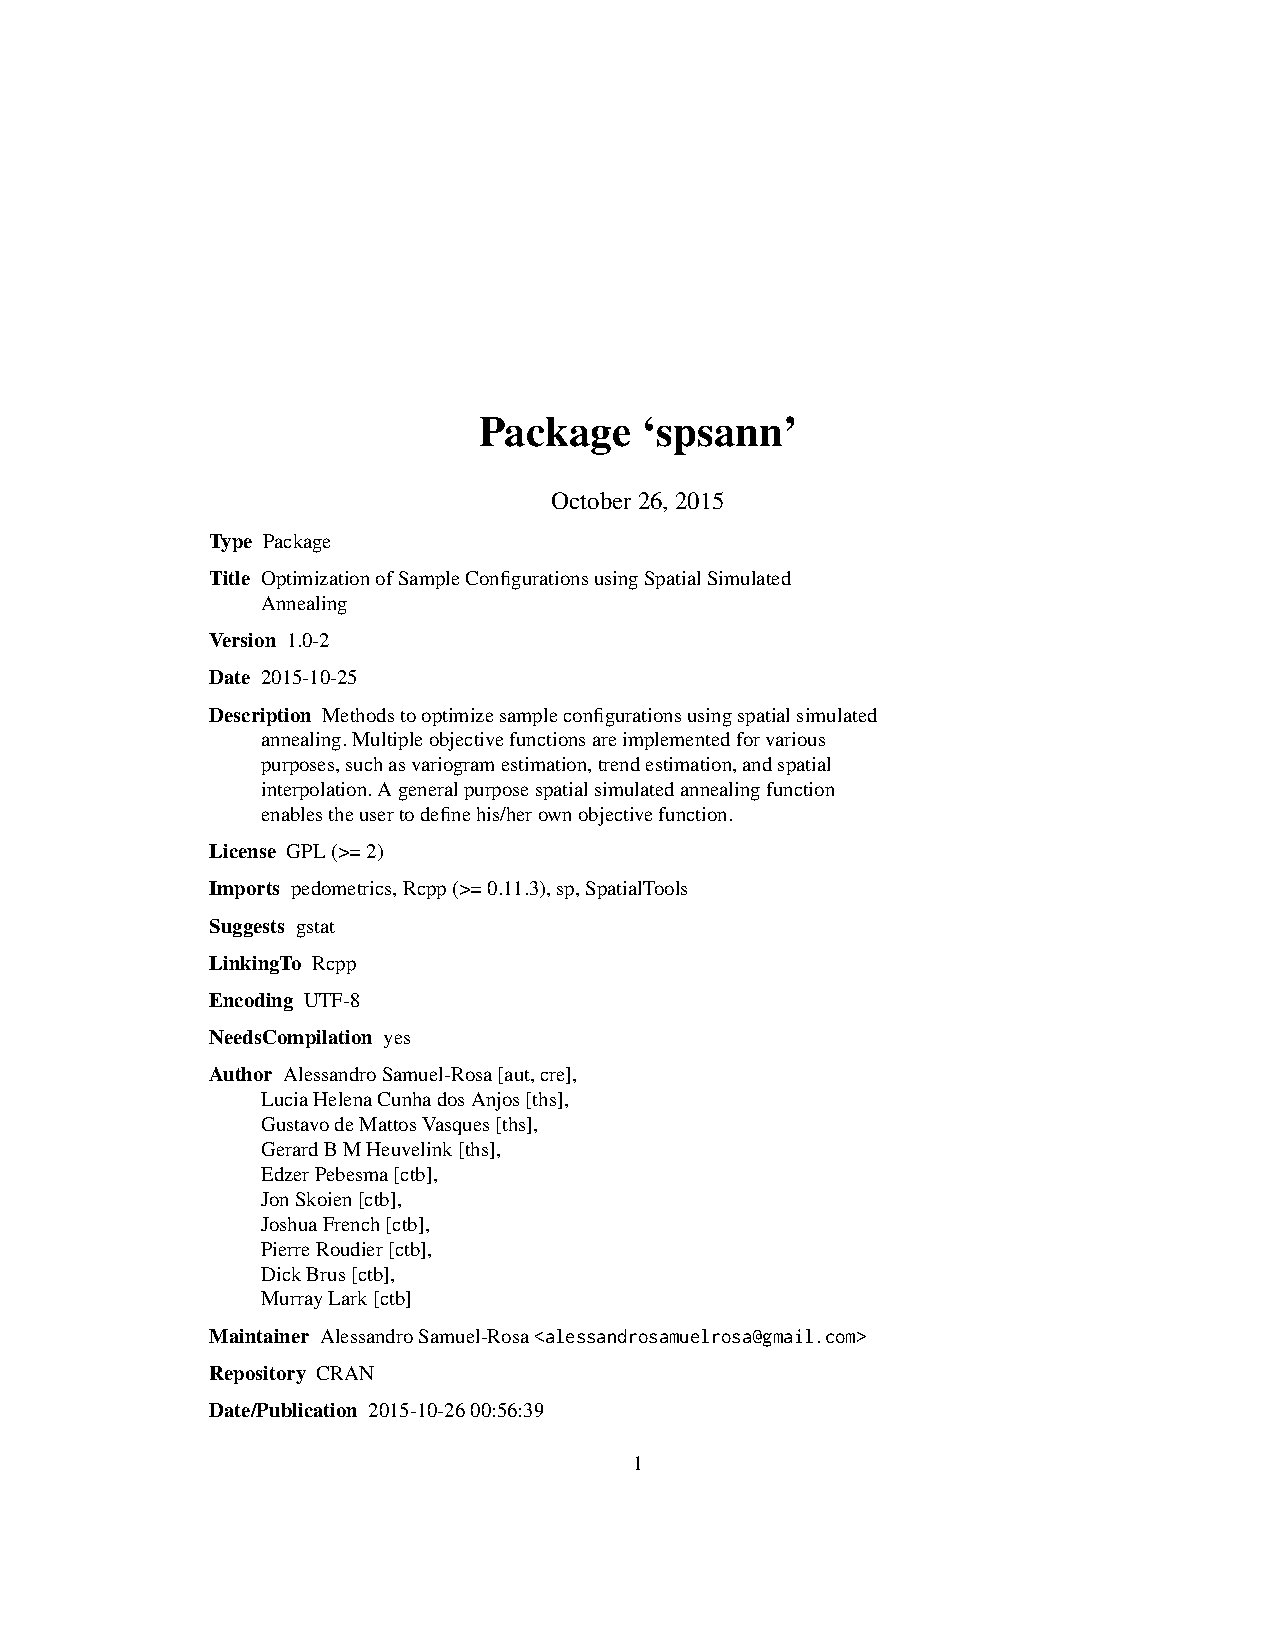
\includepdf[pages=-,pagecommand={}]{chap/spsann.pdf}

\section{Objective functions}



\section{Spatial Simulated Annealing}

\subsection{Generation Mechanism}

The \textit{generation mechanism} corresponds to the set of formal rules used 
to randomly perturb (jitter) the sample configuration to create a new solution 
out of the current one. This is done by jittering (adding random noise) the 
coordinates of the i-\textit{th} sample point.

Jittering a sample point requires the definition of the amount of random noise
that can be added to its coordinates, i.e. the area within which it can be 
moved around. In principle, this area corresponds to a rectangle centred at the 
sample point that ignores the presence of non-sampling areas (e.g. buildings 
and water bodies) and the finiteness of the sampling area. We call this the 
\textit{search graph}.

Choosing a candidate location within the search graph can be done in two 
different ways. The first method uses uses an \textit{infinite} set of candidate 
locations, that is, any location within the search graph can be selected as the 
candidate location for the sample point. After a candidate location is selected, 
it is necessary to check if it falls within the sampling area but does not fall
within a non-sampling area. clearly, this method is computationally demanding,
the reason why it is not implemented in the \textbf{spsann}-package.

The second method is more efficient because it first identifies the set of 
\textit{effective} candidate locations for the sample point. This is because it
uses a \textit{finite} set of candidate locations. A finite set of candidate 
locations is created by discretizing the sampling region, that is, creating a 
fine grid of points that serve as candidate locations for the jittered points. 
This is the least computationally demanding jittering method because, by 
definition, the jittered point will always be inside the sampling region and out 
of non-sampling areas. The disadvantage is that not all locations in the 
sampling region can be selected as the new location for a jittered point.

Using a finite set of candidate locations has another important 
inconvenience. When a point is jittered, it may be that the new location 
already is occupied by another point. If this happens, another location has
to be iteratively sought for, say, as many times as the number of points in
the sample. In general, the more points there are in the sample, the more 
likely it is that the new location already is occupied by another point. If 
a solution is not found in a reasonable time, the point selected to be 
jittered is kept in its original location. Such a procedure is clearly 
suboptimal.

The \textbf{spsann}-package uses a more elegant method which is based on using 
a finite set of candidate locations coupled with a form of \textit{two-stage 
random sampling} as implemented in the \textbf{spcosa}-package. Because 
the candidate locations are placed on a finite regular grid, they can be 
seen as being the centre nodes of a finite set of grid cells (or pixels of 
a raster image). In the first stage, one of the 'grid cells' is selected 
with replacement, i.e. independently of already being occupied by 
another sample point. The new location for the point chosen to be jittered 
is selected within that 'grid cell' by simple random sampling. This 
method guarantees that \textit{almost} any location in the sampling region can 
be a candidate location. It also discards the need to check if the new 
location already is occupied by another point, simplifying the code and 
(possibly) speeding up the computations.
 
The size of the search graph
is reduced linearly at the end of each Markov chain. The size of the search 
graph is correlated with the concept of \textit{temperature}: a larger search 
graph is equivalent to higher temperatures, which potentially result in more 
movement or 'agitation' of the set of points.

\begin{equation}
  x_max = x_max0 - (chains_i / chains) * (x_max0 - x_min) + x_cellsize
  
  y_max = y_max0 - (chains_i / chains) * (y_max0 - y_min) + y_cellsize
\end{equation}

where $x_max0$ and $y_max0$ are the maximum allowed shifts in the x- and 
y-coordinates in the first chain, $x_min$ and $y_min$ are the minimum 
required shifts in the x- and y-coordinates, $x_max$ and $y_max$ are the
maximum allowed shifts in the x- and y-coordinates during the next chain, 
$chains$ and $chain_i$ are the total and current chains, and $x_cellsize$ and
$y_cellsize$ are the grid spacing in the x- and y-coordinates.

\subsection{Annealing Schedule}

The \textit{annealing schedule} corresponds to a set of formal rules that 
determine how the probability of accepting inferior system configurations is 
decreased as the search for the globally optimum system configuration evolves.
